% Cholesky Decomposition
\section{$\mathbf{A} = \mathbf{L}\mathbf{L}^{\dagger}$ Cholesky Decomposition}
\label{sec:cholesky}

The Cholesky Decomposition exists when a matrix is hermitian and positive-definite. It expresses the matrix $\mathbf{A}$ as:

\begin{equation}
\mathbf{A} = \mathbf{L}\mathbf{L^\dagger}
\end{equation}

Where $\mathbf{L}$ is a lower-triangular matrix with positive, real diagonal entries. When $\mathbf{A}$ is real, then so is $\mathbf{L}$. The Cholesky decomposition enables fast solution of a linear system, but it can also be used to create correlated random variables in Monte Carlo simulations. 

\subsection{Creating Correlated Random Variables}
Let $\mathbf{u}_t$ be a vector of uncorrelated samples with mean 0 and 	standard deviation 1. If the covariance matrix of the system to be simulated is  $\mathbf{\Sigma}$ with Cholesky decomposition $\mathbf{\Sigma} = \mathbf{LL}^\dagger$, then the vector $\mathbf{v}_t = \mathbf{Lu}_t$ has the desired covariance.

\begin{figure}
\centering
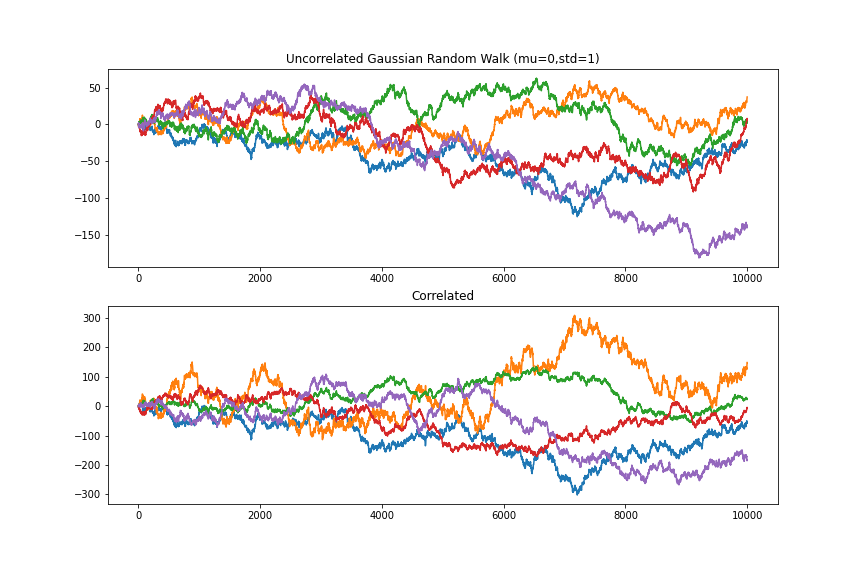
\includegraphics[scale=0.5]{cholesky1.png}
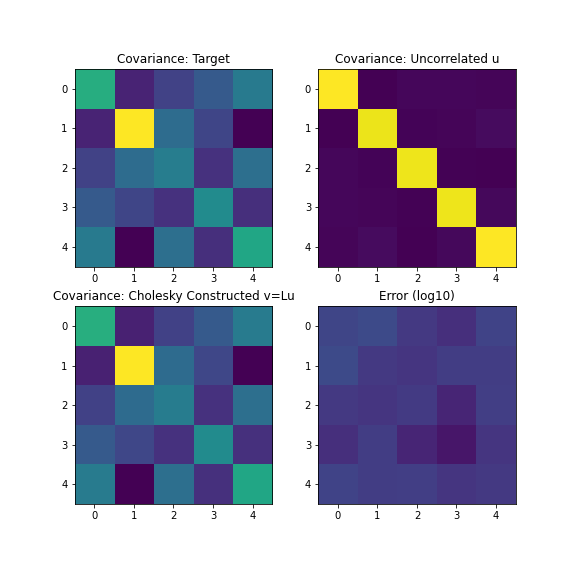
\includegraphics[scale=0.5]{cholesky2.png}
\caption{Creating correlated random variables from uncorrelated random variables using the Cholesky decomposition of the covariance matrix. The 5 uncorrelated random variables are sampled from a standard normal distribution. It is difficult to see a difference between the correlated and uncorrelated random walks.}
\end{figure}

